\chapter{\RU{Работа с числами с плавающей запятой используя SIMD}
\EN{Working with float point numbers using SIMD}}

\label{floating_SIMD}
\index{IEEE 754}
\index{SIMD}
\index{SSE}
\index{SSE2}
\RU{Разумеется, FPU остался в x86-совместимых процессорах в то время, когда ввели расширения \ac{SIMD}}
\EN{Of course, \ac{FPU} remained in x86-compatible processors, when \ac{SIMD} extensions were added}.

\ac{SIMD}-\RU{расширения}\EN{extensions} (SSE2) \RU{позволяют удобнее работать с числами с плавающей 
запятой}\EN{offers more easy way to work with float-point numbers}.

\RU{Формат чисел остается тот же}\EN{Number format remaining the same} (IEEE 754).

\index{x86-64}
\RU{Так что современные компиляторы (включая те, что компилируют под x86-64) 
обычно используют \ac{SIMD}-инструкции вместо FPU-инструкций.}\EN{So, modern compilers (including those generating
for x86-64) usually uses \ac{SIMD}-instructions instead of FPU ones.}

\RU{Это, можно сказать, хорошая новость, потому что работать с ними легче}
\EN{It can be said, it's a good news, because it's easier to work with them}.

\RU{Примеры будем использовать из секции о FPU}\EN{We will reuse here examples from the FPU section} \ref{sec:FPU}.

\section{\RU{Простой пример}\EN{Simple example}}

\lstinputlisting{patterns/12_FPU/1_simple/simple.c}

\subsection{x64}

\lstinputlisting[caption=MSVC 2012 x64 /Ox]{patterns/205_floating_SIMD/simple_MSVC_2012_x64_Ox.asm}

\RU{Собственно, входные значения с плавающей запятой передаются через регистры \XMM{0}-\XMM{3}, 
а остальные --- через стек}\EN{Input floating point values are passed in \XMM{0}-\XMM{3} registers,
all the rest---via stack}
\footnote{\href{http://msdn.microsoft.com/en-us/library/zthk2dkh.aspx}{MSDN: Parameter Passing}}.

$a$ \RU{передается через}\EN{is passed in} \XMM{0}, $b$\EMDASH{}\RU{через}\EN{via} \XMM{1}.
\RU{Но XMM-регистры (как мы уже знаем из секции о \ac{SIMD}\ref{SIMD_x86}) 128-битные, 
а значения типа \Tdouble --- 64-битные,
так что используется только младшая половина регистра}
\EN{XMM-registers are 128-bit (as we know from the section about \ac{SIMD}\ref{SIMD_x86}), 
but \Tdouble values---64 bit ones, so only lower register half is used}.

\index{x86!\Instructions!DIVSD}
\TT{DIVSD} \RU{это SSE-инструкия, означает}\EN{is SSE-instruction, meaning} 
``Divide Scalar Double-Precision Floating-Point Values'', 
\RU{и просто делит значение типа \Tdouble на другое, лежащие в младших половинах операндов}\EN{it just divides
one value of \Tdouble type by another, stored in the lower halves of operands}.

\RU{Константы закодированы компилятором в формате IEEE 754}\EN{Constants are encoded by compiler in IEEE 754 format}.

\index{x86!\Instructions!MULSD}
\index{x86!\Instructions!ADDSD}
\TT{MULSD} \AndENRU \TT{ADDSD} \RU{работают так же, только производят умножение и сложение}
\EN{works just as the same, but doing multiplication and addition}.

\RU{Результат работы ф-ции типа \Tdouble ф-ция оставляет в регистре \XMM{0}}
\EN{The result of \Tdouble type the function leaves in \XMM{0} register}.\\
\\
\RU{Как работает неоптимизирующий MSVC}\EN{That is how non-optimizing MSVC works}:

\lstinputlisting[caption=MSVC 2012 x64]{patterns/205_floating_SIMD/simple_MSVC_2012_x64.asm}

\index{Shadow space}
\RU{Чуть более избыточно}\EN{Slightly redundant}. 
\RU{Входные аргументы сохраняются в}\EN{Input arguments are saved in} ``shadow space'' (\ref{shadow_space}), 
\RU{причем, только младшие половины регистров, т.е., только 64-битные значения типа \Tdouble}
\EN{but only lower register halves, i.e., only 64-bit values of \Tdouble type}.\\
\\
\RU{Результат работы компилятора GCC точно такой же}\EN{GCC produces very same code}.

\subsection{x86}

\RU{Я скомпилировал этот пример также и под x86. MSVC 2012 даже генерируя под x86, использует 
SSE2-инструкции:}\EN{I also compiled this example for x86. Despite the fact of generating for x86, 
MSVC 2012 use SSE2-instructions:}

\lstinputlisting[caption=MSVC 2012 x86]{patterns/205_floating_SIMD/simple_MSVC_2012_x86.asm}

\lstinputlisting[caption=MSVC 2012 x86 /Ox]{patterns/205_floating_SIMD/simple_MSVC_2012_x86_Ox.asm}

\RU{Код почти такой же, правда есть пара отличий связанных с соглашениями о вызовах:}
\EN{It's almost the same code, however, there are couple differences related to calling conventions:}
1) \RU{аргументы передаются не в XMM-регистрах, а через стек, как и прежде, в примерах с FPU (\ref{sec:FPU});}
\EN{arguments are passed not in XMM registers, but in stack, like in FPU examples (\ref{sec:FPU});}
2) \RU{результат работы ф-ции возвращается через \ST{0} --- для этого он через стек
(через локальную переменную \TT{tv}) копируется из XMM-регистра в \ST{0}.}
\EN{function result is returned in \ST{0} --- in order to do so, it's copied
(through local variable \TT{tv}) from one of XMM-registers into \ST{0}.}

\RU{Попробуем соптимизированный пример в}\EN{Let's try optimized example in} \olly:
\figref{fig:FPU_SIMD_simple_olly1},
\figref{fig:FPU_SIMD_simple_olly2},
\figref{fig:FPU_SIMD_simple_olly3},
\figref{fig:FPU_SIMD_simple_olly4},
\figref{fig:FPU_SIMD_simple_olly5}.

\RU{Видно что \olly показывает XMM-регистры как пары чисел в формате \Tdouble,
но используется только \IT{младшая} часть.}
\EN{We see that \olly shows XMM-reigsters as \Tdouble number pairs,
but only \IT{lower} part is used.}
\RU{Должно быть, \olly показывает их именно так, потому что сейчас исполняются SSE2-инструкции
с суффиксом \TT{-SD}.}
\EN{Apparently, \olly shows them in that format because SSE2-instructions (suffixed with \TT{-SD}) 
are executed right now.}
\RU{Но конечно же, можно переключить отображение значений в регистрах и посмотреть содержимое
как 4 \Tfloat{}-числа или просто как 16 байт.}
\EN{But of course, it's possible to switch register format and to see its contents as
4 \Tfloat{}-numbers or just as 16 bytes.}

\begin{figure}[H]
\centering
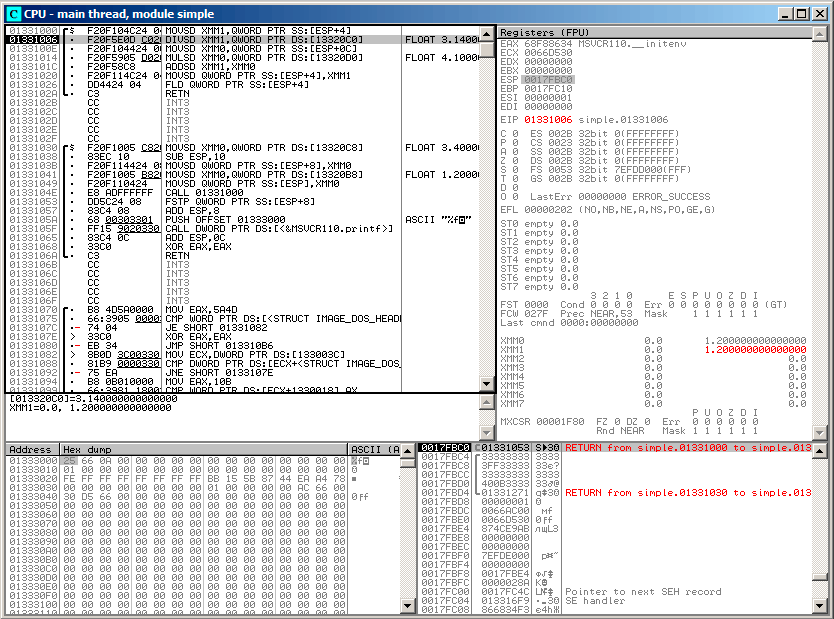
\includegraphics[scale=\FigScale]{patterns/205_floating_SIMD/simple_olly1.png}
\caption{\olly: \TT{MOVSD} \RU{загрузила значение}\EN{loads value of} $a$ \RU{в}\EN{into} \XMM{1}}
\label{fig:FPU_SIMD_simple_olly1}
\end{figure}

\begin{figure}[H]
\centering
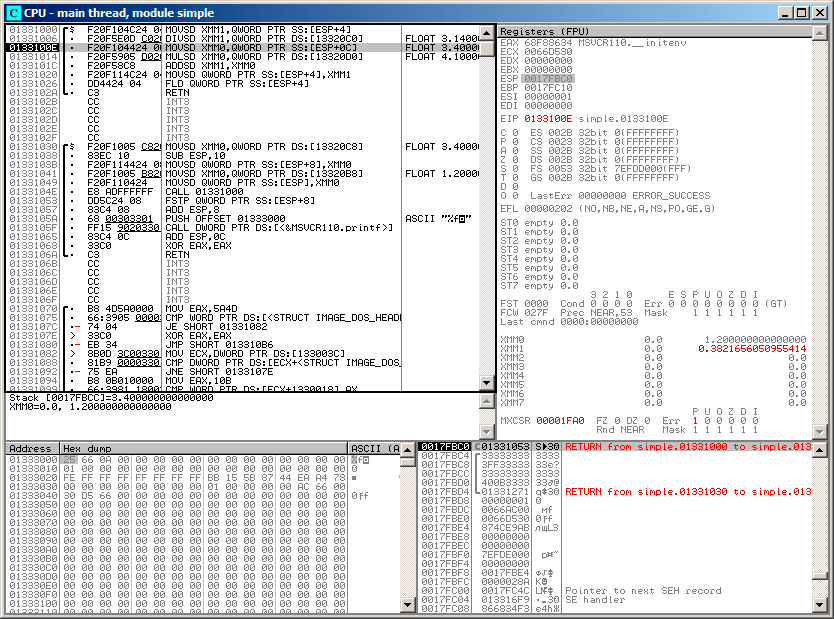
\includegraphics[scale=\FigScale]{patterns/205_floating_SIMD/simple_olly2.png}
\caption{\olly: \TT{DIVSD} \RU{вычислила}\EN{calculated} \gls{quotient} 
\RU{и оставила его в}\EN{and stored it in} \XMM{1}}
\label{fig:FPU_SIMD_simple_olly2}
\end{figure}

\begin{figure}[H]
\centering
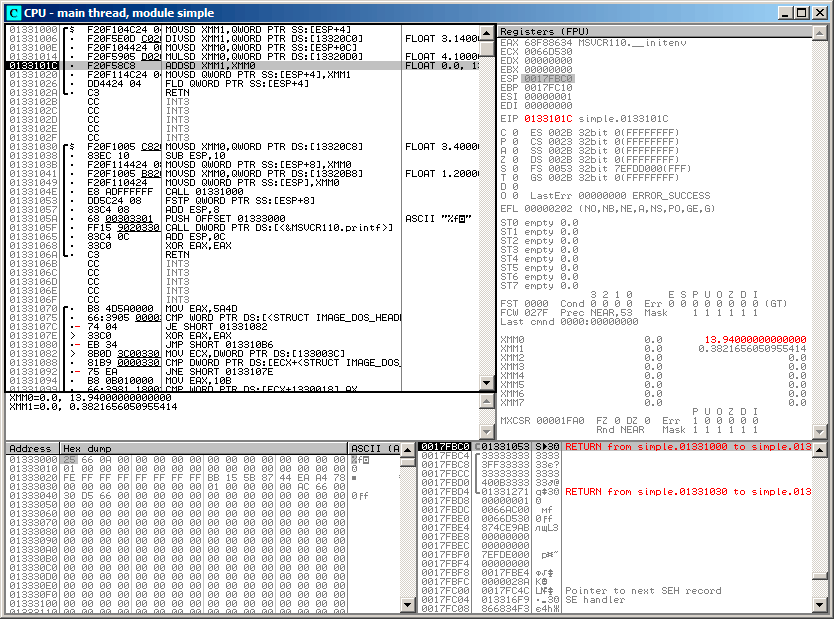
\includegraphics[scale=\FigScale]{patterns/205_floating_SIMD/simple_olly3.png}
\caption{\olly: \TT{MULSD} \RU{вычислила}\EN{calculated} \gls{product} \RU{и оставила его в}\EN{and stored it
in} \XMM{0}}
\label{fig:FPU_SIMD_simple_olly3}
\end{figure}

\begin{figure}[H]
\centering
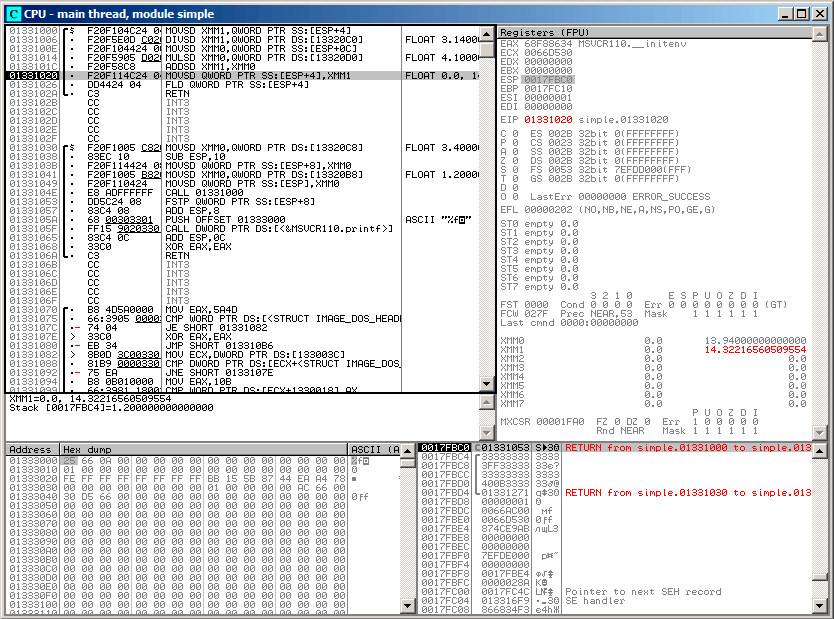
\includegraphics[scale=\FigScale]{patterns/205_floating_SIMD/simple_olly4.png}
\caption{\olly: \TT{ADDSD} \RU{прибавила значение в}\EN{adds value in} \XMM{0} \RU{к}\EN{to} \XMM{1}}
\label{fig:FPU_SIMD_simple_olly4}
\end{figure}

\begin{figure}[H]
\centering
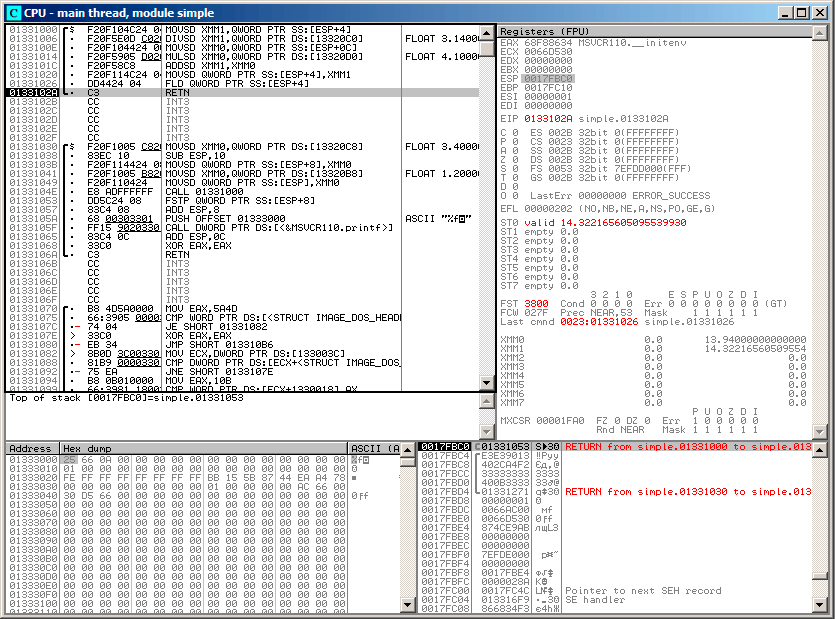
\includegraphics[scale=\FigScale]{patterns/205_floating_SIMD/simple_olly5.png}
\caption{\olly: \FLD \RU{оставляет результат ф-ции в}\EN{left function result in} \ST{0}}
\label{fig:FPU_SIMD_simple_olly5}
\end{figure}

\section{\RU{Передача чисел с плавающей запятой в аргументах}\EN{Passing floating point number via arguments}}

\lstinputlisting{patterns/12_FPU/2_passing_floats/pow.c}

\RU{Они передаются в младших половинах регистров}\EN{They are passed in lower halves
of the} \XMM{0}-\XMM{3}\EN{ registers}.

\lstinputlisting[caption=MSVC 2012 x64 /Ox]{patterns/205_floating_SIMD/pow_MSVC_2012_x64_Ox.asm}

\index{x86!\Instructions!MOVSD}
\index{x86!\Instructions!MOVSDX}
\RU{Инструкции}\EN{There are no} \TT{MOVSDX} \RU{нет в документации от}\EN{instruction in} 
Intel\cite{Intel} \AndENRU AMD\cite{AMD}\EN{ manuals}, 
\RU{там она называется просто}\EN{it is called there just} \TT{MOVSD}.
\RU{Таким образом, в процессорах x86 две инструкции с одинаковым именем}\EN{So there are two instructions
sharing the same name in x86} (\RU{о второй}\EN{about other}: \ref{REP_MOVSx}).
\RU{Возможно, в Microsoft решили избежать
путанницы и переименовали инструкцию в}\EN{Apparently, Microsoft developers wanted to get rid of mess,
so they renamed it into} \TT{MOVSDX}.
\RU{Она просто загружает значение в младшую половину XMM-регистра}\EN{It just loads a value into
lower half of XMM-register}.

\RU{Ф-ция }\TT{pow()} \RU{берет аргументы из}\EN{takes arguments from} \XMM{0} \AndENRU \XMM{1}, 
\RU{и возвращает результат в}\EN{and returning result in} \XMM{0}.
\RU{Далее он перекладывается в}\EN{It is then moved into} \RDX \ForENRU \printf. 
\RU{Почему}\EN{Why}? 
\RU{Честно говоря, не знаю, может быть, это потому что}\EN{Honestly speaking, I don't know, maybe because} 
\printf\EMDASH{}\RU{ф-ция с переменным количеством аргументов}\EN{is a variable arguments function}?

\lstinputlisting[caption=GCC 4.4.6 x64 \Othree]{patterns/205_floating_SIMD/pow_GCC446_x64_O3_\LANG.s}

GCC \RU{работает понятнее}\EN{making more clear result}. 
\RU{Значение для}\EN{Value for} \printf \RU{передается в}\EN{is passed in} \XMM{0}. 
\RU{Кстати, вот тот случай, когда в}\EN{By the way, here is a case when 1 is written into} \EAX
\ForENRU \printf \RU{записывается 1 --- это значит, что будет передан один аргумент в векторных регистрах, 
так того требует стандарт}\EN{---this mean that one argument will be passed in vector registers,
just as the standard requires} \cite{SysVABI}.

\section{\RU{Пример с сравнением}\EN{Comparison example}}

\lstinputlisting{patterns/12_FPU/3_comparison/d_max.c}

\subsection{x64}

\lstinputlisting[caption=MSVC 2012 x64 /Ox]{patterns/205_floating_SIMD/d_max_MSVC_2012_x64_Ox.asm}

\Optimizing MSVC \RU{генерирует очень понятный код}\EN{generates very easy code to understand}.

\index{x86!\Instructions!COMISD}
\RU{Инструкция }\TT{COMISD} \RU{это}\EN{is} ``Compare Scalar Ordered Double-Precision Floating-Point 
Values and Set EFLAGS''. \RU{Собственно, это она и делает}\EN{Essentially, that is what it does}.\\
\\
\NonOptimizing MSVC \RU{генерирует более избыточно, но тоже всё понятно}\EN{generates more redundant code,
but it is still not hard to understand}:

\lstinputlisting[caption=MSVC 2012 x64]{patterns/205_floating_SIMD/d_max_MSVC_2012_x64.asm}

\index{x86!\Instructions!MAXSD}
\RU{А вот}\EN{However,} GCC 4.4.6 \RU{дошел в оптимизации дальше и применил инструкцию}
\EN{did more optimizing and used the} \TT{MAXSD} (``Return Maximum Scalar 
Double-Precision  Floating-Point Value'')\RU{, которая просто выбирает максимальное значение}\EN{ instruction,
which just choose maximal value}!

\lstinputlisting[caption=GCC 4.4.6 x64 \Othree]{patterns/205_floating_SIMD/d_max_GCC446_x64_O3.s}

\subsection{x86}

\RU{Скомпилируем этот пример в MSVC 2012 с включенной оптимизацией:}
\EN{Let's compile this example in MSVC 2012 with optimization turned on:}

\lstinputlisting[caption=MSVC 2012 x86 /Ox]{patterns/205_floating_SIMD/d_max_MSVC_2012_x86_Ox.asm}

\RU{Всё то же самое, только значения}\EN{Almost the same, but values of} $a$ \AndENRU $b$ 
\RU{берутся из стека, а результат функции оставляется в}\EN{are taked from stack and function result 
is left in} \ST{0}.

\RU{Если загрузить этот пример в}\EN{If to load this example in} \olly, 
\RU{увидим как инструкция}\EN{we will see how} \TT{COMISD} \RU{сравнивает значения и устанавливает/сбрасывает
флаги}\EN{instruction compares values and set/clear} \CF \AndENRU \PF\EN{ flags}: \figref{fig:FPU_SIMD_d_max_olly}.

\begin{figure}[H]
\centering
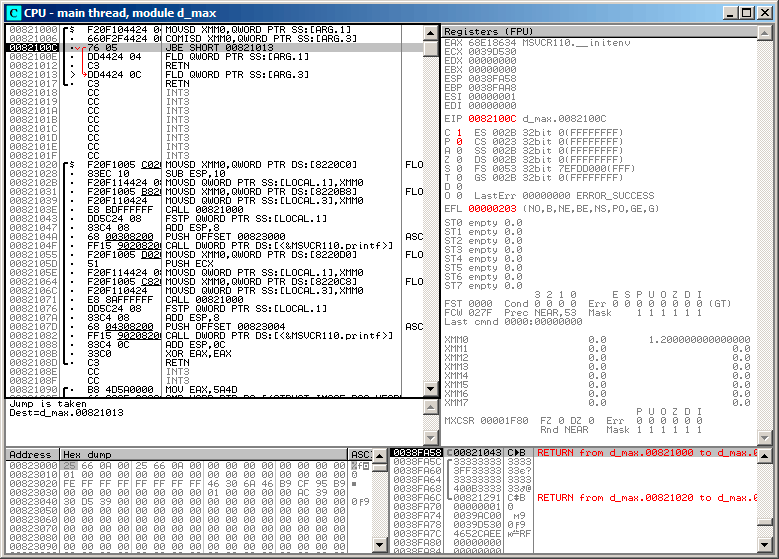
\includegraphics[scale=\FigScale]{patterns/205_floating_SIMD/d_max_olly.png}
\caption{\olly: \TT{COMISD} \RU{изменила флаги}\EN{changed} \CF \AndENRU \PF\EN{ flags}}
\label{fig:FPU_SIMD_d_max_olly}
\end{figure}

\section{\RU{Итог}\EN{Summary}}

\RU{Во всех приведенных примерах, в XMM-регистрах используется только младшая половина регистра, там
хранится значение в формате IEEE 754}\EN{Only lower half of XMM-registers are used in all examples here, 
a number in IEEE 754 format is stored there}.

\RU{Собственно, все инструкции с суффиксом}\EN{Essentially, all instructions prefixed by} 
\TT{-SD} (``Scalar Double-Precision'')\EMDASH{}\RU{это инструкции для работы с числами с плавающей 
запятой в формате IEEE 754, 
хранящиеся в младшей 64-битной половине XMM-регистра}\EN{are instructions working with float point numbers
in IEEE 754 format stored in the lower 64-bit half of XMM-register}.

\RU{Всё удобнее чем это было в FPU, видимо, сказывается тот факт что расширения 
SIMD развивались не так хаотично как FPU в прошлом}
\EN{And it is easier than FPU, apparently because SIMD extensions were evolved not as chaotic as FPU in the past}.
\RU{Стековая модель регистров не используется}\EN{Stack register model is not used}.

\index{x86!\Instructions!ADDSS}
\index{x86!\Instructions!MOVSS}
\index{x86!\Instructions!COMISS}
\RU{Если вы попробуете заменить в этих примерах}\EN{If you would try to replace} \Tdouble \RU{на}\EN{to} \Tfloat
\RU{, то инструкции будут использоваться те же,
только с суффиксом}\EN{in these examples, the same instructions will be used, but prefixed with} \TT{-SS} 
(``Scalar Single-Precision''), \RU{например}\EN{for example}, \TT{MOVSS}, \TT{COMISS}, \TT{ADDSS}, \RU{итд}\EN{etc}.

``Scalar'' \RU{означает что SIMD-регистр будет хранить только одно значение, вместо нескольких}\EN{mean that
SIMD-register will contain only one value instead of several}.
\RU{Инструкции, работающие с несколькими значениями в регистре одновременно, имеют ``Packed'' в названии}
\EN{Instructions working with several values in a register simultaneously, has ``Packed'' in the name}.

\RU{Нужно также обратить внимание, что SSE2-инструкции работают с 64-битными числами (\Tdouble) в формате IEEE 754,
в то время как внутреннее представление в FPU --- 80-битные числа.}
\EN{Needless to say that SSE2-instructions works with 64-bit IEEE 754 numbers (\Tdouble),
while internal representation of float-point numbers in FPU --- 80-bit numbers.}
\RU{Поэтому ошибок округления (\IT{round-off error}) в FPU может быть меньше чем в SSE2.}
\EN{Hence, FPU may produce less round-off errors.}
